\section{Evaluation}
\label{sec:evaluation}

\subsection{Experiments setup}

\parab{Testbed setup.}
The testbed consists of 8 servers, each equipped with 4 NVIDIA GeForce RTX 3090 GPUs, 40 CPU cores (Intel(R) Xeon(R) Gold 5218R CPU @ 2.10GHz), 128GB RAM, and two ConnectX-5 100Gbps NIC. The servers are connected via NVIDIA SN2700 Ethernet switches. Within each server, the GPUs communicate via PCIe Gen 3.0. All servers run Ubuntu 22.04 with CUDA 12.8, PyTorch 2.8.0, and NCCL 2.28. we configure a prefill cluster comprising 16 GPUs, while decode workers are provisioned separately. For simplicity, we limit the decode output length to one token, since it does not affect TTFT.

\parab{Simulation setup.}
Our simulator is built upon Vidur~\cite{agrawal2024vidur} and the flow-level simulator flowsim~\cite{FlowSim2024}. We extend Vidur to support the Mixtral model with expert and sequence parallelism, as well as PD disaggregation with KV-cache reuse. The simulation workflow begins with offline profiling of operator latencies via Vidur profiler. At runtime, we employ a unified event-driven mechanism: Vidur simulates the LLM serving behavior to generate computation and communication tasks, while flowsim parser the communication task and trigger the underlying network events. Crucially, both computation events and network events are processed within a single event queue to ensure correctness. By default, we simulate a 256-server cluster with a 1:1 prefill-decode worker ratio, managed by a KV-cache aware scheduler similar to Dynamo~\cite{NVIDIA_Dynamo}.  Each server hosts eight GPUs interconnected via NVSwitch (900 GB/s) and eight NICs, connected via a 1:1 fat-tree network with link bandwidth 200Gbps. The latency profiles are calibrated based on NVIDIA A100 GPU.

\parab{Metrics.}
We primarily evaluate Time-to-First-Token (TTFT) and its Service Level Objective (SLO) attainment rate. Following the methodology in~\cite{patke2024queue,hongsola,stojkovic2025dynamollm}, we define the SLO threshold as $3\times$ the TTFT measured under low-load conditions by default. We also evaluate microbenchmarks such as the collective completion time (CCT) and request earliness to help interpret the observed performance gains.

\subsection{Testbed Experiments}
\label{sec:evaluation:testbed}

\begin{figure}[t!]
    \centering
    \begin{subfigure}[t]{0.48\linewidth}
        \centering
        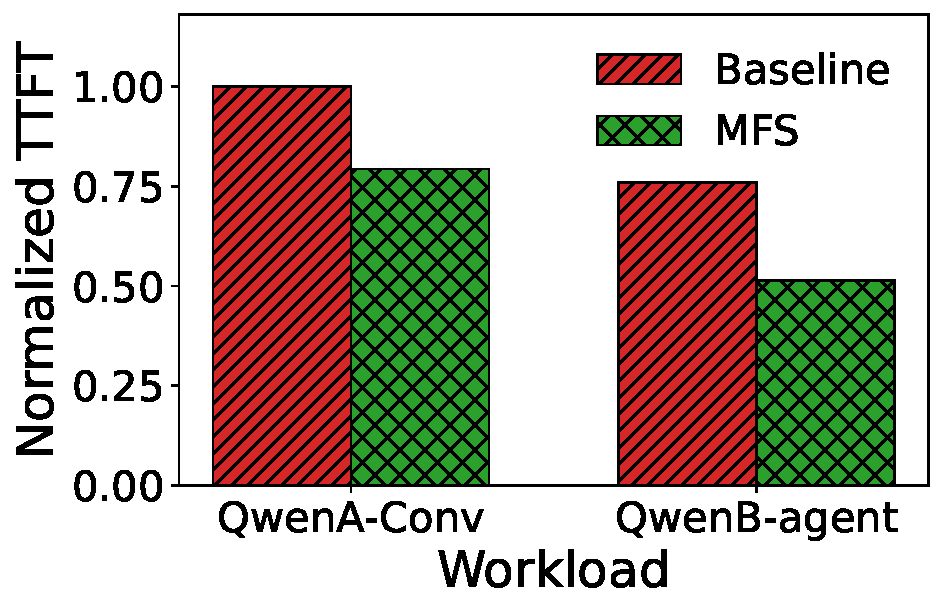
\includegraphics[width=\linewidth]{figures/evaluation/testbed/mixtral_TTFT_mfs.pdf}
        \caption{Normalized TTFT.}
        \label{fig:evaluation:testbed:ttft}
    \end{subfigure}
    \hfill
    \begin{subfigure}[t]{0.48\linewidth}
        \centering
        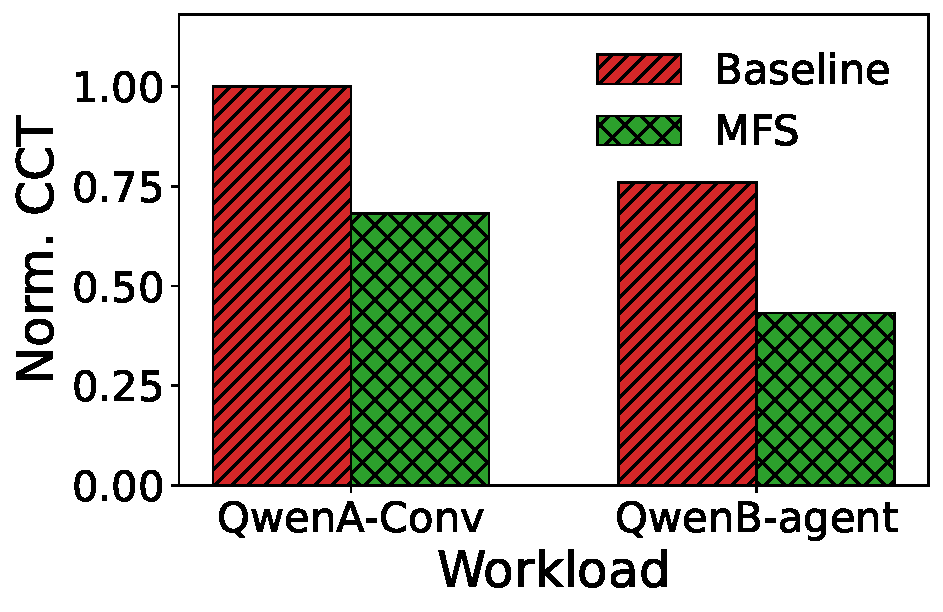
\includegraphics[width=\linewidth]{figures/evaluation/testbed/mixtral_alltoall_mfs.pdf}
        \caption{Normalized CCT.}
        \label{fig:evaluation:testbed:cct}
    \end{subfigure}
    \hfill
    \caption{[Testbed] Mixtral-8x7B}
    \label{fig:evaluation:testbed}
\end{figure}


\begin{figure*}[ht!]
    \centering
    \begin{subfigure}[t]{0.9\linewidth}
        \centering
        
\includegraphics[width=0.9\linewidth]{figures/evaluation/SLO_legend_MFS.pdf}
    \end{subfigure}
    \vspace{-0.5em}
    \begin{subfigure}[b]{0.24\linewidth}
        \centering
        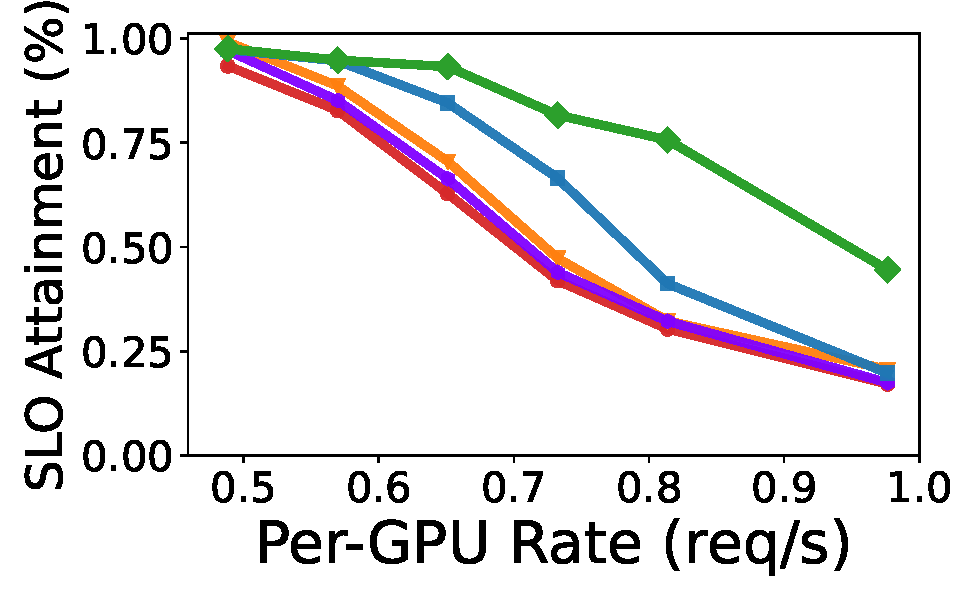
\includegraphics[width=\linewidth]{figures/evaluation/sim_qwenA/qwenA_mixtral8x22B_bw200.pdf}
        \caption{Mixtral-8x22B}
        \label{fig:evaluation:qwenA:mixtral_200}
    \end{subfigure}
    \hfill
    \begin{subfigure}[b]{0.24\linewidth}
        \centering
        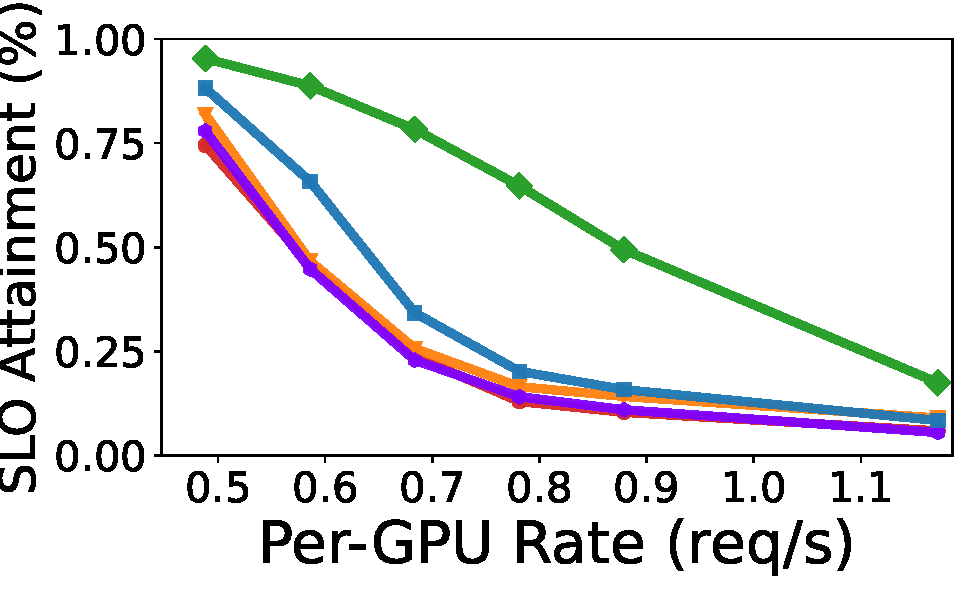
\includegraphics[width=\linewidth]{figures/evaluation/sim_qwenA/qwenA_dbrx_bw200.pdf}
        \caption{DBRX}
        \label{fig:evaluation:qwenA:dbrx_200}
    \end{subfigure}
    \hfill
    \begin{subfigure}[b]{0.24\linewidth}
        \centering
        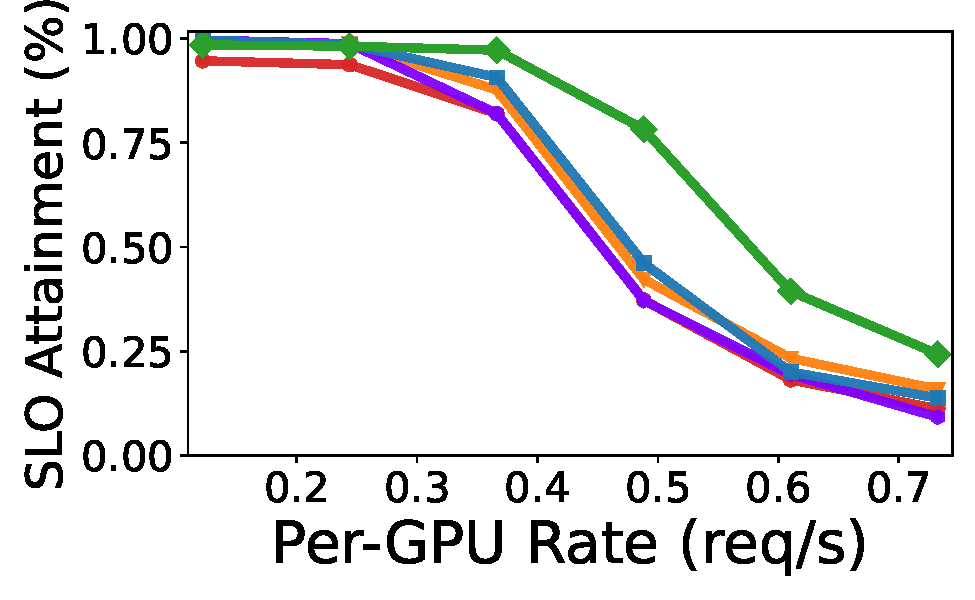
\includegraphics[width=\linewidth]{figures/evaluation/sim_qwenA/qwenA_coder_bw200.pdf}
        \caption{Qwen3-Coder}
        \label{fig:evaluation:qwenA:qwencoder_200}
    \end{subfigure}
    \hfill
    \begin{subfigure}[b]{0.24\linewidth}
        \centering
        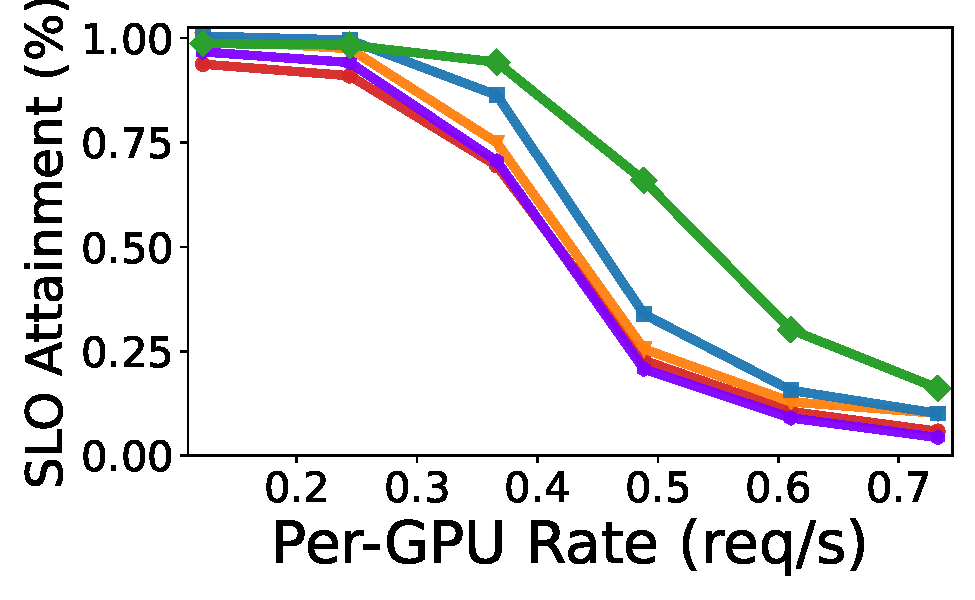
\includegraphics[width=\linewidth]{figures/evaluation/sim_qwenA/qwenA_grok2_bw200.pdf}
        \caption{Grok2}
        \label{fig:evaluation:qwenA:grok2_200}
    \end{subfigure}
    \caption{[Simulation] Performance on conversation workload (QwenA)
    }
    \label{fig:evaluation:qwenA}
\end{figure*}

\input{sections/fig_code/evaluation/sim_qwenB}

\parab{Model and workload.}
In the testbed experiment, We evaluate the Mistral 8x7B~\cite{mixtral7b} MoE model (FP16, top-$k$=2), configured with a tensor parallelism (TP) degree of 1 and expert parallelism (EP) of 8. For the workload, we utilize two production traces derived from Qwen~\cite{qwen_bailian_traces}. QwenA-Conv represents a \textit{conversation workload} with an average sequence length of 2k tokens and a 50\% prompt reuse rate. QwenB-agent represents an \textit{agent workload}, characterized by an average length of 1k tokens and a higher reuse rate of 65\%. Request arrivals follow a Poisson process, where we vary the requests per second (RPS) to modulate system load. Due to testbed capacity limits, we clip the first 512 requests of each trace as a warm-up phase and use the subsequent 1024 requests for evaluation.

Figure~\ref{fig:evaluation:testbed} reports how \sys{} on QwenA-Conv and QwenB-Agent workload. We configure vLLM with 8192 batched tokens and set the per-GPU request rate to one request per second. \sys{} significantly reduces TTFT across both workloads, optimizing the mean TTFT by 20.7\% (1.26×) on QwenA-Conv and 32.3\% (1.48×) on QwenB-Agent. The TTFT reduction is primarily driven by faster completion of computation-blocking collectives. As shown by the all-to-all completion time (CCT), \sys{} shortens stage-2 communication by 31.9\% (1.47×) on QwenA-Conv and 43.1\% (1.76×) on QwenB-Agent. These collectives lie directly on the critical path of prefill execution: delaying them immediately stalls GPU computation and inflates end-to-end latency.


\subsection{Large-Scale Simulations}

In the large-scale simulations, we expand the evaluation scope to cover a diverse spectrum of production-grade architectures and workloads.
\begin{itemize}[leftmargin=*]
    \item We examine a comprehensive set of mainstream MoE models with expert parallelism, ranging from architectures with large but few experts (e.g., Mixtral 8x22B~\cite{mixtral22b} and Grok-2~\cite{grok}, configured with TP=4, EP=8) to models with small but many experts (e.g., DBRX~\cite{dbrx} with TP=2, EP=16, and Qwen3-Coder~\cite{qwen-coder} with TP=1, EP=32). These models are deployed with 32-GPU instance utilizing a hybrid parallelism strategy. We evaluate these MoE models using Qwen conversation and agent traces to represent typical interactive behaviors.
    \item We further assess the effectiveness of \sys{} on dense models with sequence parallelism~\cite{ringattention}. We evaluate the Llama~\cite{llama} model configured with a 1M token context window. In this setup, the model is deployed on 16-GPU instance using TP=4 and SP=4. We pair this model with the Mooncake dataset~\cite{mooncake} to simulate real-world conversation and agent workloads characterized by similar reuse ratios ($\sim40\%$, $\sim65\%$) and extended context lengths ($\sim15k$, $\sim9k$).
\end{itemize}

\parab{Baselines.} We compare \sys{} against four classic flow scheduling policies:
\begin{itemize}[leftmargin=*]
    \item \textbf{Fair Sharing} enforces max-min fairness among concurrent flows by allocating bandwidth equally, regardless of flow sizes or deadlines.
    \item \textbf{Shortest Job First (SJF)} minimizes average flow completion time by strictly prioritizing flows with smaller flow sizes.
    \item \textbf{Earliest Deadline First (EDF)} prioritizes flows with explicit deadlines. Since application-level deadlines do not directly translate to individual network flow deadlines, it applies fair sharing for flows with implicit deadlines.
    \item \textbf{Karuna~\cite{karuna}} allocates the minimum required bandwidth to flows with deadlines to ensure on-time completion, while scheduling the remaining flows using SJF.
\end{itemize}

\parab{End-to-End TTFT SLO Attainment.} We evaluate the end-to-end TTFT SLO attainment under varying request rates across diverse models and workloads. As shown in Fig~\ref{fig:evaluation:qwenA}, \ref{fig:evaluation:qwenB}, and \ref{fig:evaluation:sp}, \sys{} consistently outperforms state-of-the-art baselines across all scenarios.

Figure~\ref{fig:evaluation:qwenA} details the performance of \sys{} on conversation workloads for diverse MoE models. Specifically, under high request rates, \sys{} achieves $1.4\times$--$1.8\times$ higher SLO attainment for Mixtral (Fig.~\ref{fig:evaluation:qwenA:mixtral_200}), Qwen Coder (Fig.~\ref{fig:evaluation:qwenA:qwencoder_200}) and Grok (Fig.~\ref{fig:evaluation:qwenA:grok2_200}), and up to $2.4\times$ for DBRX (Fig.~\ref{fig:evaluation:qwenA:dbrx_200}). Furthermore, \sys{} can sustain $1.17\times$--$1.46\times$ higher request rates than the strongest baseline (Karuna) while maintaining the similar SLO attainment. In conversation workload, a small fraction of tail requests necessitates large KV-cache movements, which precipitate contention across Stage~1 to Stage~3 under high load. \sys{} outperform baselines significantly since it successfully coordinates multi-stage contention. Among the baselines, Karuna performs relatively better because it \emph{happens to} defer non-urgent Stage~3 traffic and provides partial relief; however, without explicit multi-stage coordination, it eventually succumbs to contention as other baselines.

Figure~\ref{fig:evaluation:qwenB} details the performance of \sys{} on agent workloads for diverse MoE models. Focusing on the mid-to-high load regime, \sys{} achieves $1.4\times$--$1.7\times$ higher SLO attainment for Grok-2 and Mixtral, and reaches $2.0\times$ for DBRX and Qwen-Coder. Furthermore, \sys{} sustains $1.2\times$ higher request rates for Grok-2, $\sim1.3\times$ for Mixtral and Qwen-Coder, and up to $1.4\times$ for DBRX compared to the Karuna. Compared to conversation traces, agent requests have shorter prompt length but exhibit higher average reuse rates, with multiple concurrent requests sharing identical prefixes. This pattern induces severe one-to-many sender-side contention, which primarily concentrates on Stage~1 and Stage~2 as multiple workers simultaneously contend for the same cached states. \sys{} effectively mitigates this contention by protecting urgent flows without requiring precise laxity. Notably, the performance gap between Karuna and other baselines narrows in this scenario. When contention is not dominated by Stage~3 traffic, Karuna falls back to SJF (deadline is implicit) to schedule Stage~1 and Stage~2 flows; however, being unaware of stage semantics, this approach still exposes tight requests to SLO violations as other baselines.

\begin{figure}[t!]
    \centering
    \begin{subfigure}[b]{0.48\linewidth}
        \centering
        
\includegraphics[width=\linewidth]{figures/evaluation/sim_mc_conv/llama3_bw200_mfs.pdf}
        \caption{Conversation workload }
        \label{fig:evaluation:sp:conv}
    \end{subfigure}
    \hfill
    \begin{subfigure}[b]{0.48\linewidth}
        \centering
        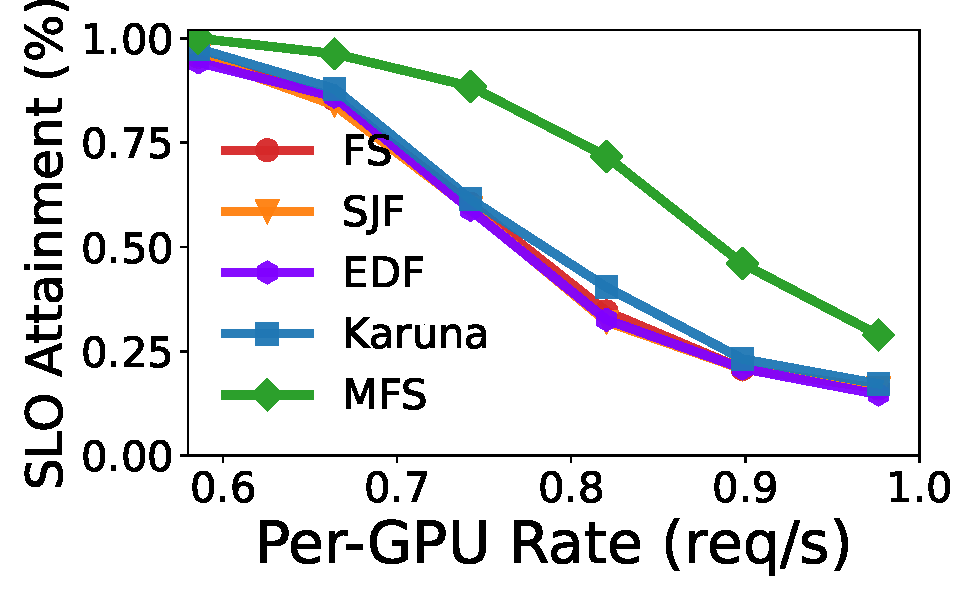
\includegraphics[width=\linewidth]{figures/evaluation/sim_mc_agent/llama3_bw200_mfs.pdf}
        \caption{Agent workload}
        \label{fig:evaluation:sp:agent}
    \end{subfigure}
    \hfill
    \vspace{-0.3cm}
    \caption{[simulation] llama3-8B (Mooncake dataset)}
    \label{fig:evaluation:sp}
\end{figure}

Figure~\ref{fig:evaluation:sp} details the performance of \sys{} on two representative long-context workloads using the Llama3-8B model with Sequence Parallelism (SP). For the Mooncake dataset, the conversation and agent workloads follow request patterns similar to those in the Qwen experiments (e.g., reuse ratios, access patterns), but feature significantly longer context lengths. In the conversation workload (Fig.~\ref{fig:evaluation:sp}a), \sys{} demonstrates robust performance under increasing load, achieving $1.3\times$--$1.6\times$ higher SLO attainment against Karuna. This advantage is further amplified in the agent workload(Fig.~\ref{fig:evaluation:sp}b), where \sys{} attains $1.4\times$--$1.9\times$ higher SLO attainment and supports up to $1.15\times$ higher per-gpu request rates given tight SLO budget.

\parab{Breaking down the performance gains.} We further conduct micro-benchmarks to analyze the source of the gains. As shown in Figure~\ref{fig:evaluation:qwenA:dbrx:mb} and Figure~\ref{fig:evaluation:sp_mb}, \sys{} successfully (i) minimizes Collective Completion Time (the non-overlapping communication latency) to shorten the prefill makespan, and (ii) regulates earliness to protect truly urgent requests under contention.

Figure~\ref{fig:evaluation:qwenA:dbrx:mb} breaks down the performance gains that lead to the $2.2\times$ higher SLO attainment achieved by \sys{} on the DBRX model.
The first source of improvement comes from reduced execution time during the prefill phase. Specifically, \sys{} lowers the average CCT of expert parallel by $52\%$ (Figure~\ref{fig:evaluation:qwenA:dbrx:cascading}). This reduction is mainly attributed to our stage-aware policy, which protects flows that block computation while deferring non-critical traffic to exploit available slack for overlap.
As a result, \sys{} significantly shortens the prefill makespan by lowering the effective communication overhead.

\begin{figure}[t!]
    \centering
    \begin{subfigure}[t]{0.48\linewidth}
        \centering
        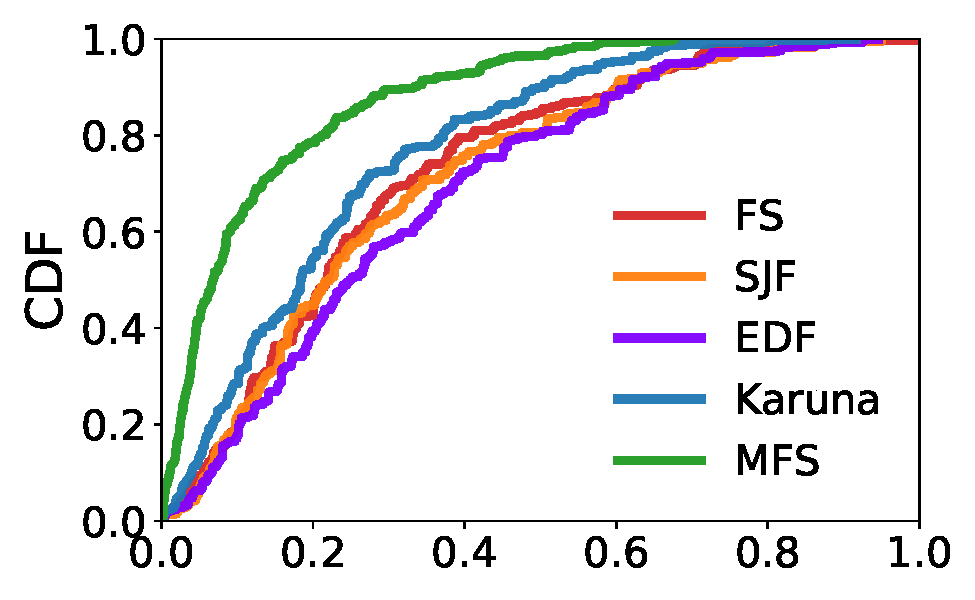
\includegraphics[width=\linewidth]{figures/evaluation/sim_qwenA/dbrx_bw200_cascading_delay_cdf_mfs.pdf}

        \caption{Normalized CCT.}
        \label{fig:evaluation:qwenA:dbrx:cascading}
    \end{subfigure}
    \hfill
    \begin{subfigure}[t]{0.48\linewidth}
        \centering
        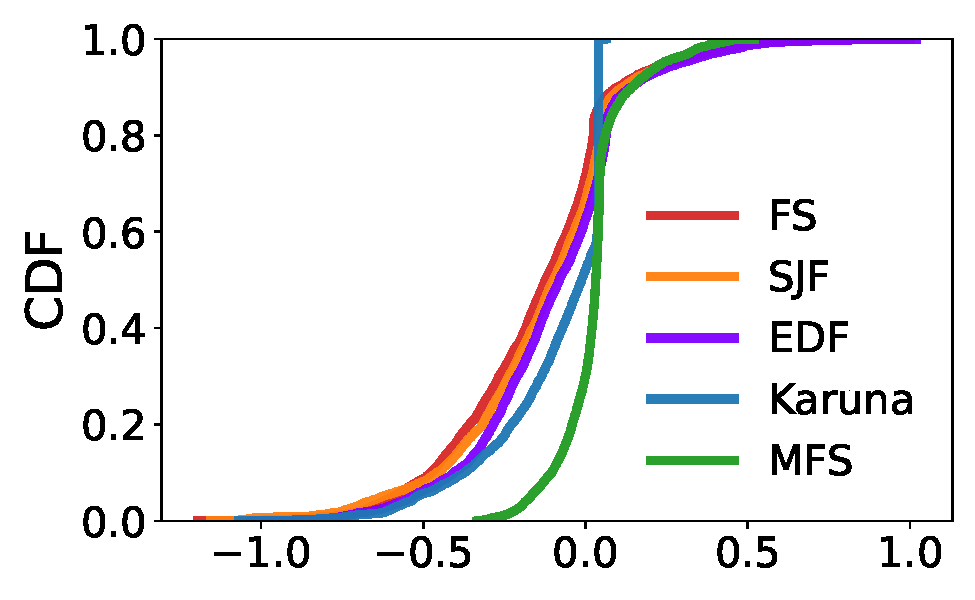
\includegraphics[width=\linewidth]{figures/evaluation/sim_qwenA/dbrx_bw200_earliness_cdf_mfs.pdf}
        \caption{Normalized earliness.}
        \label{fig:evaluation:qwenA:dbrx:earliness}
    \end{subfigure}
    \hfill
    \caption{[Simulation] Breakdown on DBRX (Qwen-A, Rate=0.7)}
    \label{fig:evaluation:qwenA:dbrx:mb}

\end{figure}

\begin{figure}[t!]
    \centering
    \begin{subfigure}[t]{0.48\linewidth}
        \centering
        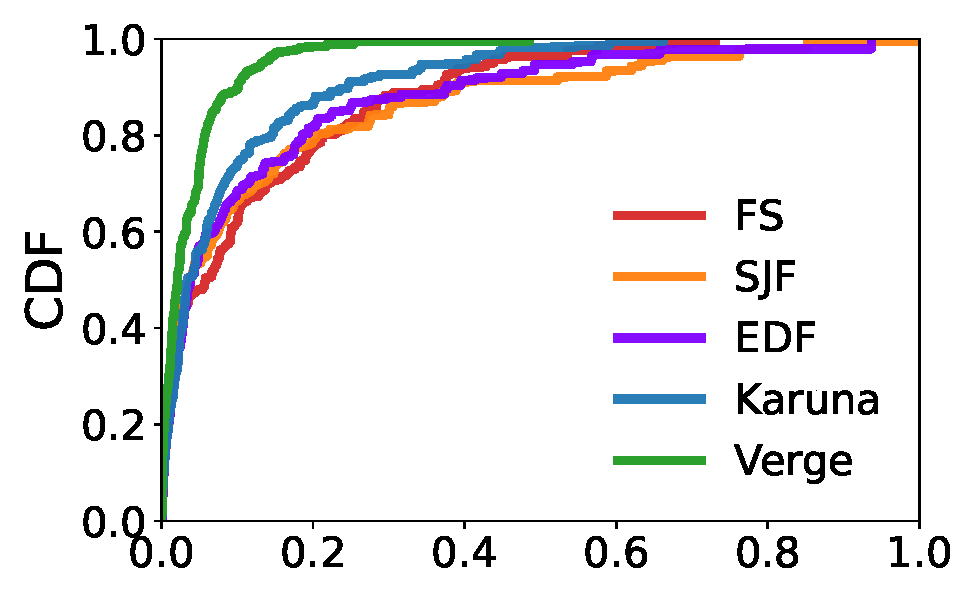
\includegraphics[width=\linewidth]{figures/evaluation/sim_mc_agent/cascading_delay_cdf.pdf}

        \caption{Normalized CCT.}
        \label{fig:evaluation:sp:cascading}
    \end{subfigure}
    \hfill
    \begin{subfigure}[t]{0.48\linewidth}
        \centering
        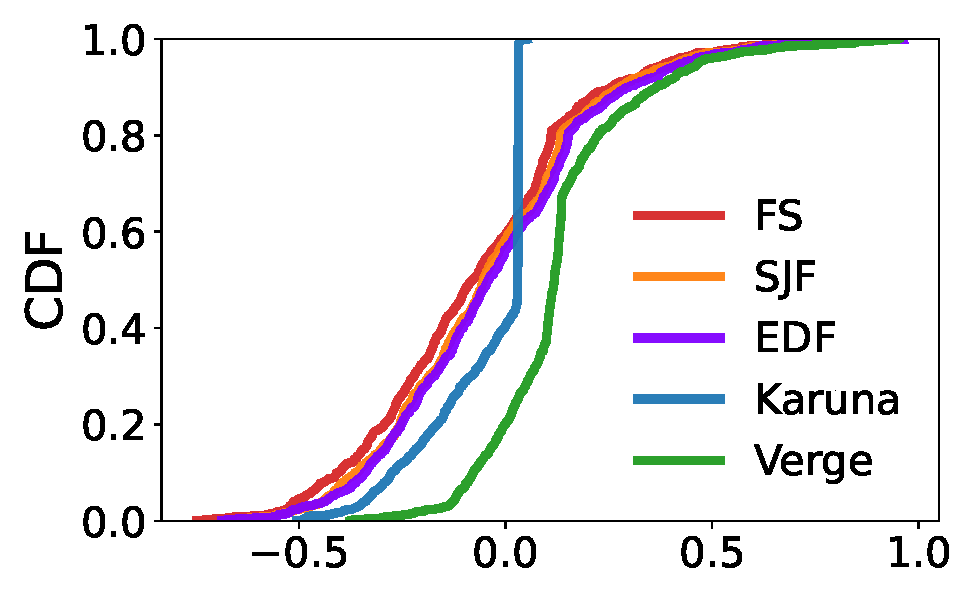
\includegraphics[width=\linewidth]{figures/evaluation/sim_mc_agent/request_earliness_cdf.pdf}

        \caption{Normalized earliness}
        \label{fig:evaluation:sp:earliness}
    \end{subfigure}
    \hfill
    \caption{[Simulation] Breakdown on Llama3 (Mooncake-Conv, Rate=0.5)}
    \label{fig:evaluation:sp_mb}
    \vspace{-0.5em}
\end{figure}


Beyond latency reduction, \sys{} further improves SLO attainment by better prioritizing truly urgent requests under contention.
We characterize this effect using \emph{earliness} of request, where large positive values indicate unnecessary early completion that can block urgent requests, while negative values correspond to deadline misses.
As shown in Figure~\ref{fig:evaluation:qwenA:dbrx:earliness}, Karuna exhibits the smallest non-negative earliness, but at the cost of a high violation risk, as it conservatively allocates near-minimal rates and fails to exploit available bandwidth.
In contrast, other baselines show much larger non-negative earliness, indicating that they schedule flows without effectively prioritizing urgency.
\sys{} reduces the non-negative portion of earliness by $42\%$ comparing with FS, SJF, EDF. By deferring Stage~3 flows to complete \textit{just-in-time} and regulating early-stage traffic with a RED-based ording, \sys{} preserves resources for turely urgent requests. \sys{} adopts a priority-based scheduling that can exploit available bandwidth when no higher-priority flows are pending.

We observe a similar trend in Figure~\ref{fig:evaluation:sp_mb}.
Across both micro-benchmarks, \sys{} consistently achieves higher SLO attainment by simultaneously reducing the collective completion time of sequence parallel (Figure~\ref{fig:evaluation:sp:cascading}) and regulating earliness under contention (Figure~\ref{fig:evaluation:sp:earliness}).
These results indicate that the performance gains of \sys{} are robust across models and are not tied to a specific workload or architecture.
